%% The following is a directive for TeXShop to indicate the main file
%%!TEX root = diss.tex

\chapter{Background}
\label{ch:Background}

\section{BDI}
\label{sec:BDI}
The BDI cache introduced in \cite{bdi} is a cache that takes advantage of similarities within data lines to compress those lines into smaller sizes, in the following section we discuss the BDI cache, it's compression, structure, and operation.
\subsection{Compression}
\label{Compression}
\subsubsection{Base Delta Compression}
The authors in \cite{bdi} have observed that data lines of real world applications have a great degree of redundancy, some of the patterns observed are:
\begin{itemize}
    \item \textbf{Zeros:} a lot of cache data lines are zeros, this is a very common case because zeros are usually used to initialize data structures, they're also very common in applications that deal with sparse matrices.
    \item \textbf{Repeated Values:} This can be observed in applications that initialize large arrays to the same initial value, or in multimedia applications where adjacent pixels could hold the same colours.
    \item \textbf{Narrow Values:} Because programmers always code for the worst case and thus have to pick large data types, while in fact the majority of the values can fit in smaller narrower data types.
    \item \textbf{Similar Values:} Values that are somewhat similar but not exactly, those are values that have high entropy in their lower bits but have the same higher bits. An example would be a list of pointers that are in the same memory regions, or pixels of an image that have almost similar colours.
\end{itemize}
\begin{figure}
    \makebox[\textwidth][c]{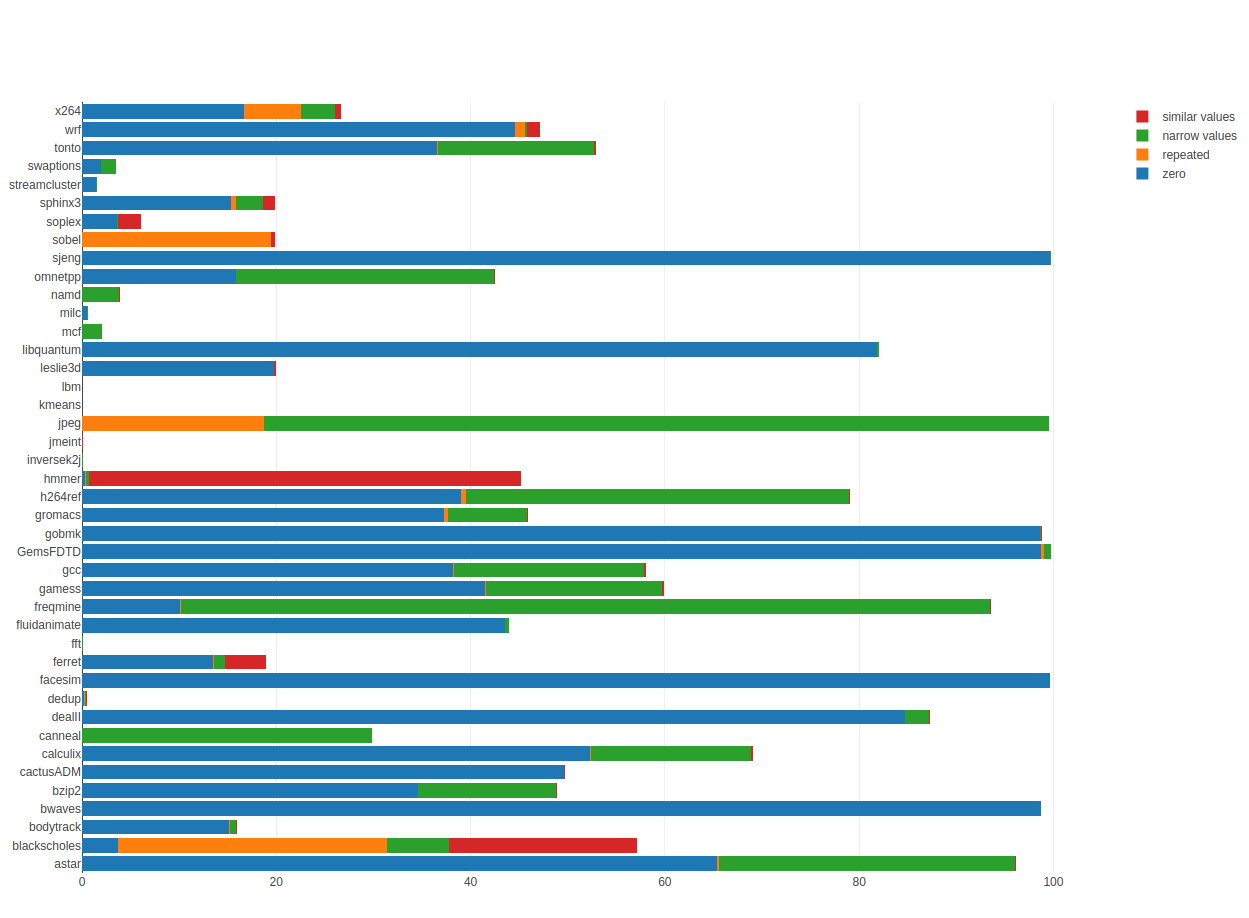
\includegraphics[width=1.5\textwidth]{BDIPotential.png}}
    \label{fig:BDIPotential}
    \caption[BDI Patterns]{The figure shows the percentage of cache lines that have one of the following patterns: zero, repeated values, narrow values, or similar values}
\end{figure}
Figure \ref{fig:BDIPotential} shows the percentage of lines where those patterns occur in a cache.
In the previously mentioned patterns, the data in a cache line granularity have a low dynamic range, the difference between values in one cache line can be represented using fewer bytes than the original data type. A compression scheme was proposed to utilize this low dynamic range, it works by representing the data line using a base value, and an array of delta values, since the delta values can be smaller in size than the original data elements, this allows for a lot of savings in the data line itself. If the delta size required to represent the delta is not smaller than the original size, the line is then incompressible and is left untouched.
Finding the right base is key to compress the data line optimally, the right base size would affect the deltas and their sizes. Since caches have no knowledge of the data types stored in them, compression is not able to identify whether a specific data line is comprised of 16 bit integers or 32 bit floats. The compression method thus has to look for the best base size, choosing one base size statically would affect the quality of compression, so the authors opted to allow three different base sizes: 2, 4 and 8 bytes that can be used and chosen from dynamically. Once a base size is chosen, the base value itself mush be found. Ideally, selecting the base value in a compressed line should be in the middle point between the minimum and the maximum values of a cache line, but that would complicate the hardware implementation so the authors opted to use the first value as base. The allowed compression and compressed sizes are shown in Figure \ref{fig:BaseDeltaCompression} and table \ref{tab:BDICompressionSizes}.
\begin{figure}
    \makebox[\textwidth][c]{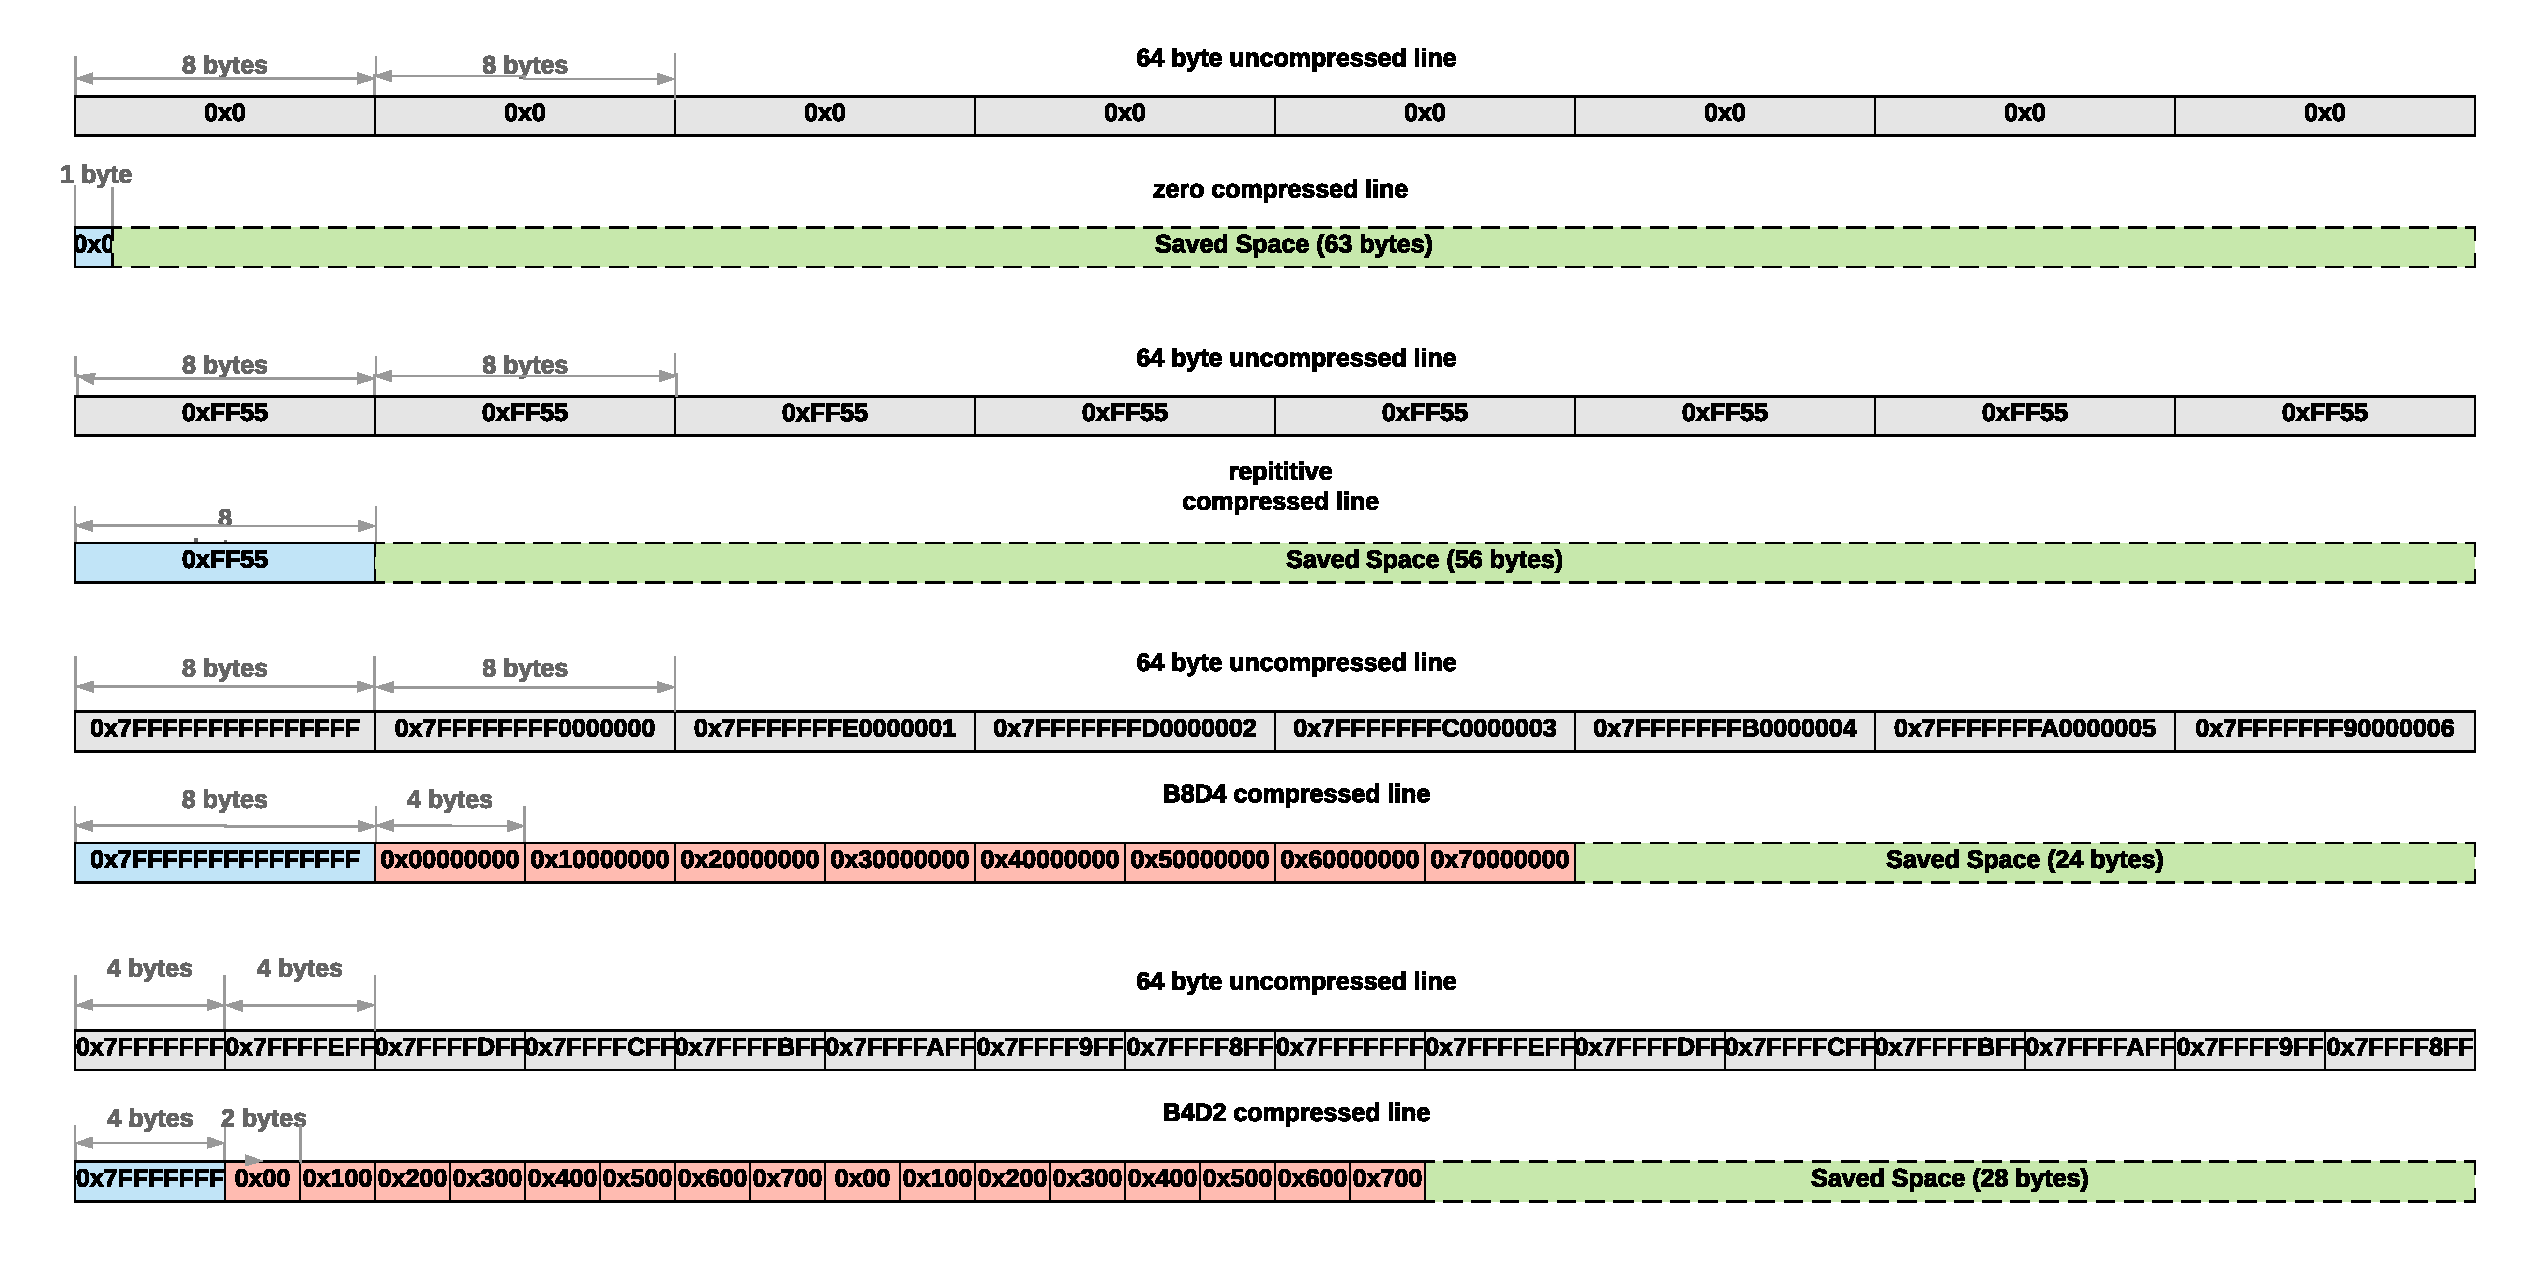
\includegraphics[width=1.5\textwidth]{BaseDeltaCompression.pdf}}
    \label{fig:BaseDeltaCompression}
    \caption[Base Delta Compression Examples]{The figure shows examples of different cases of Base Delta compression, the first two are zero and repetition line compression which are special cases, then the following cases use bases of size 8, 4, and 2}
\end{figure}
\subsubsection{Base Delta Immediate Compression}
Although one can gain a lot of compression from the base delta compression scheme, some patterns cannot be represented just by one base value, an example would be applications that use structs comprising of different data types. Because of this, allowing the base delta compression to use more than one base might help compress such lines. Based on experiments in \cite{bdi} it was clear that bases more than two do not provide much compression, so the authors selected two bases as their optimum number, but to avoid the complexity of looking for a second base when compressing a data line, the authors opted to use the second base as an implicit zero. The intuition behind this is when structs are used in applications, they're likely to contain wide values with low dynamic range (e.g. Pointers) along with narrow values, the authors observe that using an implicit zero base captures most of the compression enabled by using an arbitrary second base.
\begin{table}[]
\centering
\caption[BDI Sizes]{The table shows BDI compression sizes, all sizes are in bytes. Original line size is 64 bytes.}
\label{tab:BDICompressionSizes}
\begin{tabular}{|c|c|c|c|c|}
\hline
\textbf{Name}         & \textbf{\begin{tabular}[c]{@{}c@{}}Base\\ Size\end{tabular}} & \textbf{\begin{tabular}[c]{@{}c@{}}Delta\\ Size\end{tabular}} & \textbf{\begin{tabular}[c]{@{}c@{}}Compression\\ Size\end{tabular}} & \textbf{\begin{tabular}[c]{@{}c@{}}Compression\\ Encoding\end{tabular}} \\ \hline
\textbf{Zero}         & 1                                                            & 0                                                             & 1                                                                   & 0000                                                                    \\ \hline
\textbf{Rep}          & 8                                                            & 0                                                             & 8                                                                   & 0001                                                                    \\ \hline
\textbf{B8D1}         & 8                                                            & 1                                                             & 16                                                                  & 0010                                                                    \\ \hline
\textbf{B8D2}         & 8                                                            & 2                                                             & 24                                                                  & 0011                                                                    \\ \hline
\textbf{B8D4}         & 8                                                            & 4                                                             & 40                                                                  & 0100                                                                    \\ \hline
\textbf{B4D1}         & 4                                                            & 1                                                             & 20                                                                  & 0101                                                                    \\ \hline
\textbf{B4D2}         & 4                                                            & 2                                                             & 36                                                                  & 0110                                                                    \\ \hline
\textbf{B2D1}         & 2                                                            & 1                                                             & 34                                                                  & 0111                                                                    \\ \hline
\textbf{Uncompressed} & N/A                                                          & N/A                                                           & 64                                                                  & 1111                                                                    \\ \hline
\end{tabular}
\end{table}
\subsubsection{Compression Hardware}
\label{sssec:BDICompressionHardware}
The compression hardware used for BDI consists of eight units, two for the zero and repetitive compression schemes and six units for the three different bases with their deltas, each unit corresponds for one of the compression sizes described in Table \ref{tab:BDICompressionSizes}. Each unit outputs whether the line can be compressed in its scheme or not, and if it can be compressed it also outputs the compressed line. If multiple units can compress the line then the selection logic picks the one with the least compressed size.
A compression unit treats the line as elements of its corresponding base size, it picks the first element as the base and then subtracts all the elements from the it, if all the results can be represented in the required delta size then the line is compressed. Figure \ref{fig:BDIHardware} shows the compression hardware.
\begin{figure}
    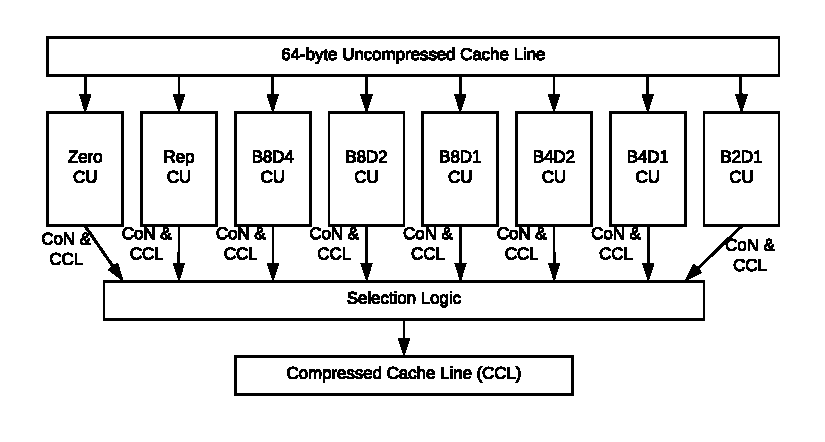
\includegraphics[width=\textwidth]{BDIHardware.pdf}
    \label{fig:BDIHardware}
    \caption[BDI Compression Hardware]{The figure shows BDI compression hardware. CU: Compression Unit, CoN: Compressed or Not?, CCL: Compressed Cache Line}
\end{figure}

\subsection{Structure}
\label{ssec:BDIStructure}
The BDI cache builds upon the conventional cache design by adding some modifications to allow compression, tags and data arrays are arranged in sets, tag sets and data sets are coupled. The BDI cache structure is shown in Figure \ref{fig:BDI}
\subsubsection{Tag Array}
\label{sssec:BDITag}
Tag arrays in a BDI cache are no different than their counterparts in a conventional cache. The tags are arranged in sets and ways. Along with its normal function, the tags also have two extra fields: The first is a compression metadata field, which describe the type of compression in the corresponding data line and a mask to distinguish which base is used for each delta. The second field is a pointer to the first segment of the current data line. Other than the addition of compression metadata and pointer no other changes happen to the tag array. There are no constraint on its organization or replacement policy.
Because BDI potentially allows more data to be stored in the same cache size, more tags are needed to address this data. The tag array has to generally have more tags than data lines otherwise no benefits come out of compression.
\subsubsection{Data Array}
\label{sssec:BDIData}
Data lines in a BDI cache are logically divided into eight fixed size segments of eight bytes each (assuming a 64 byte cache line). A compressed data line can occupy any number of segments between one and eight. The data array does not save any metadata. In that sense, the cache no longer has coupled tag and data lines but it still maintains coupled data and tag sets, i.e. A tag entry is no longer associated with a data entry in the corresponding location in the data array, but is associated with one of the segments in the corresponding set in the data array, the location of that segment depends on the compression encodings in the current selected tag set.
\begin{figure}
    \makebox[\textwidth][c]{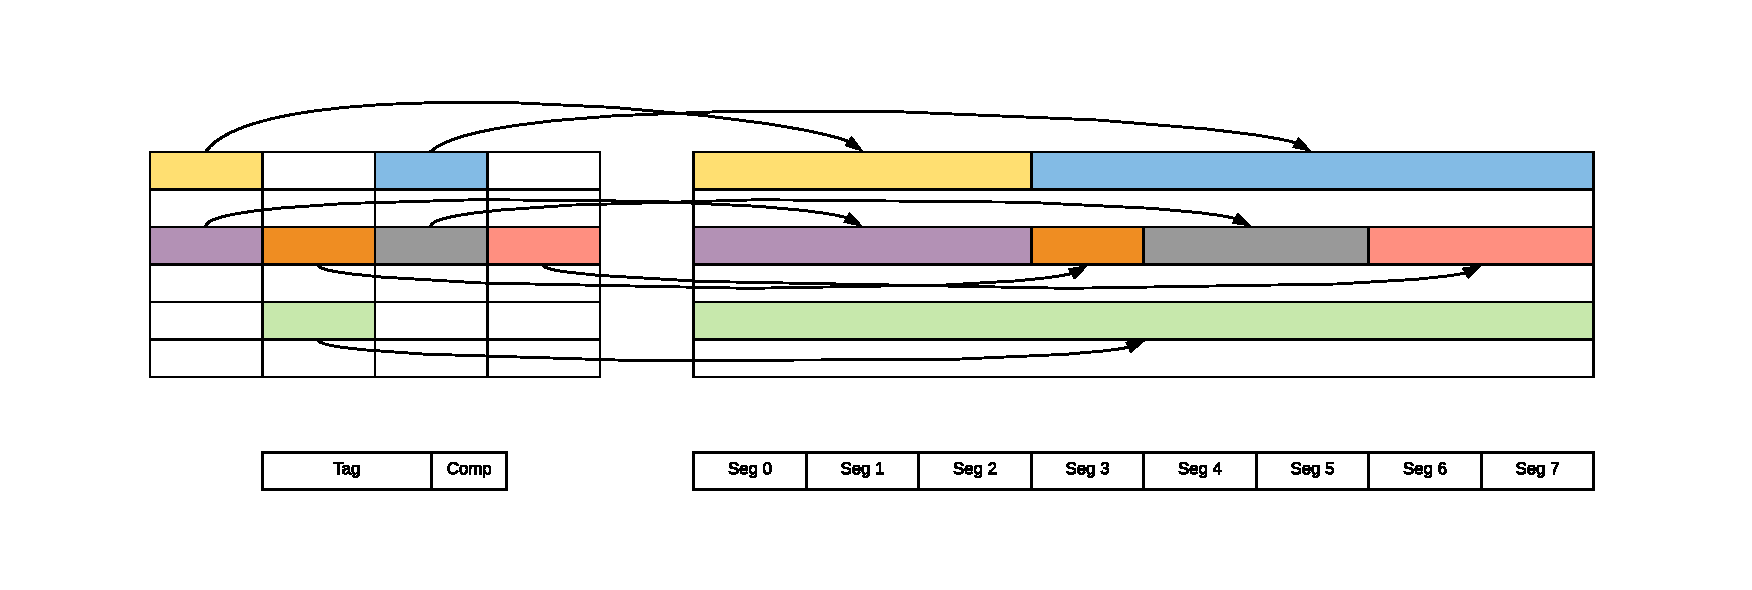
\includegraphics[width=1.5\textwidth]{BDI.pdf}}
    \label{fig:BDI}
    \caption[BDI Cache]{General structure of a BDI Cache, Tags have a compression encoding field and a segment pointer, each tag corresponds with some segments in the associated data set.}
\end{figure}

\subsection{Operations}
\label{ssec:BDIOperations}
\begin{figure}
    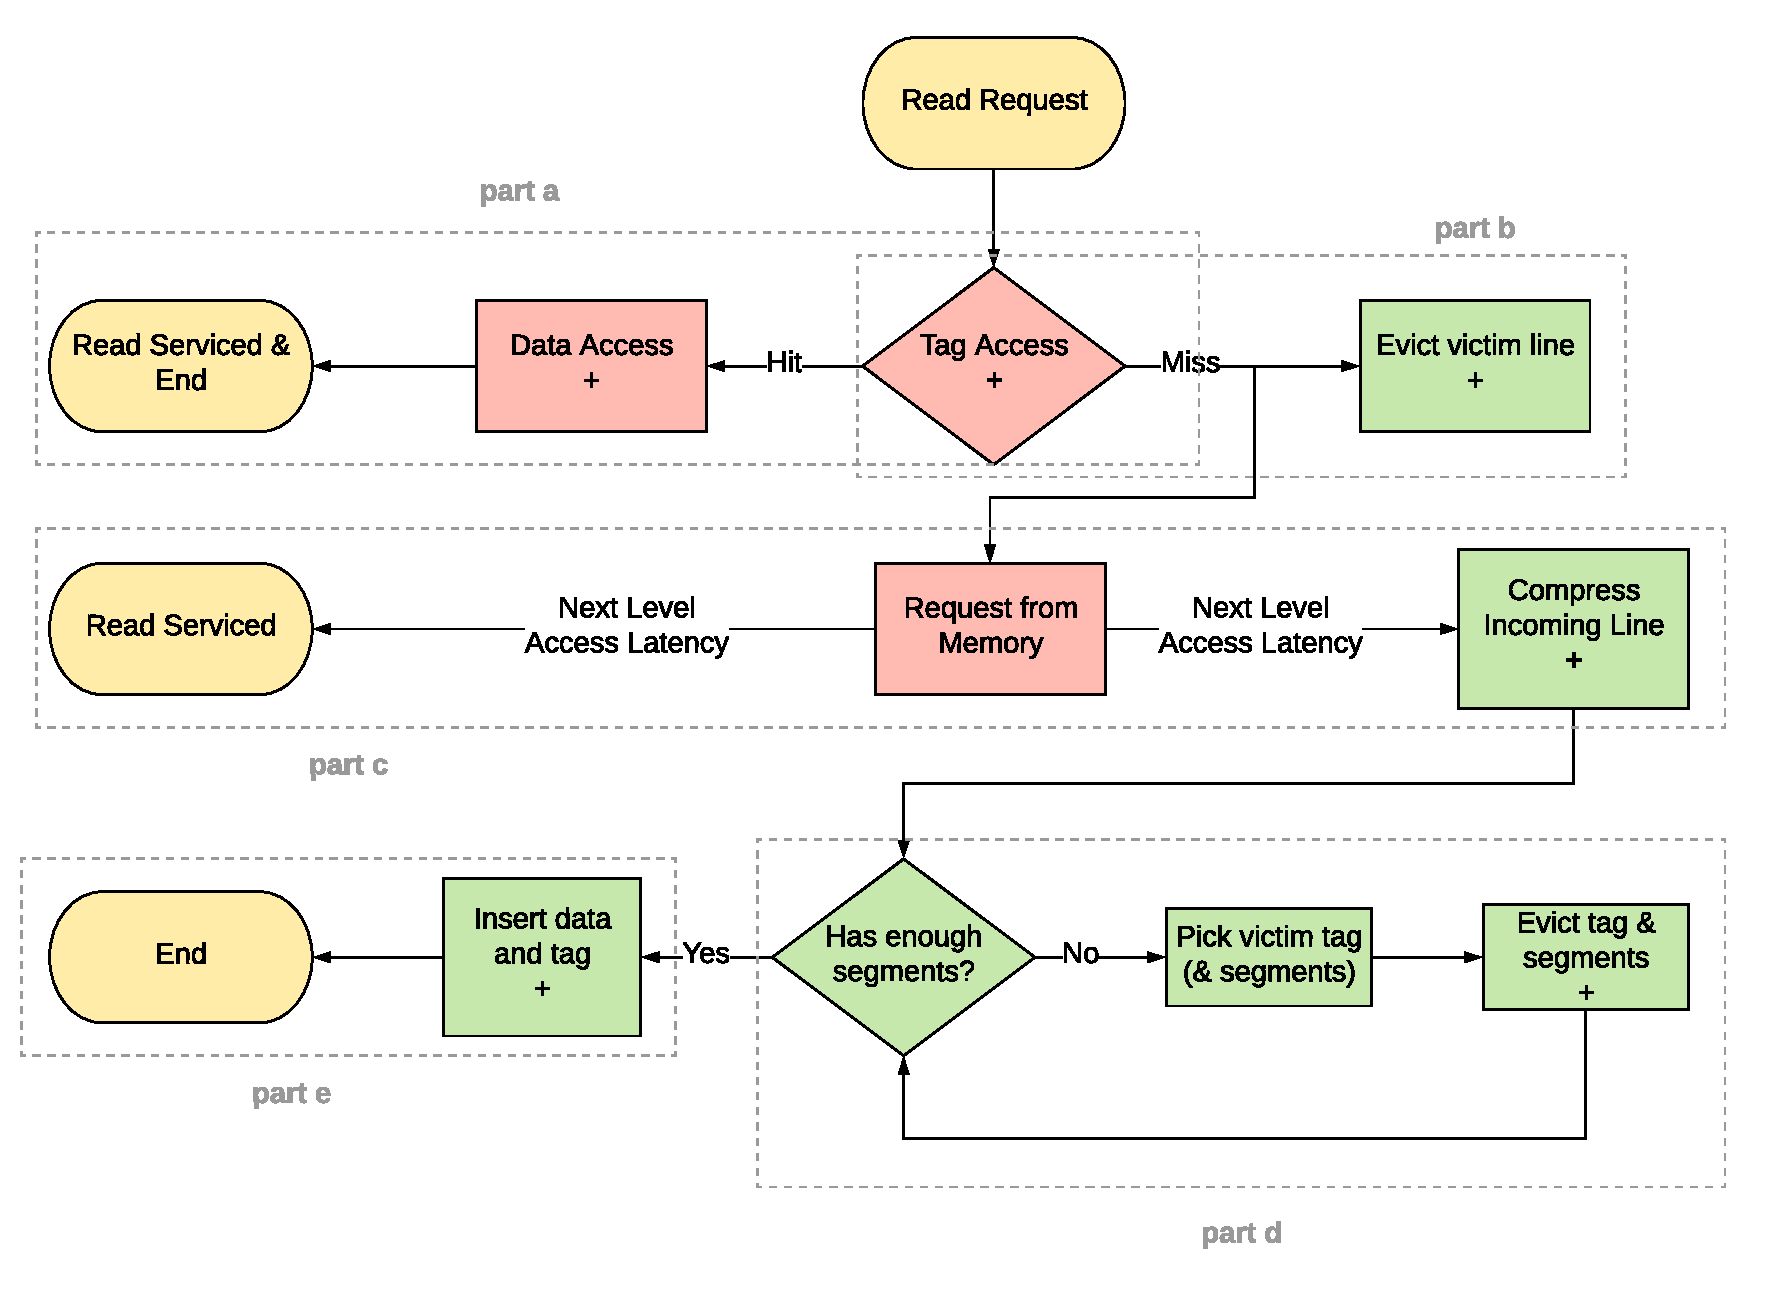
\includegraphics[width=\textwidth,height=\textheight]{BDI_Read.pdf}
    \label{fig:BDI_Read}
    \caption[BDI Read]{Read access flowchart.}
\end{figure}
\begin{figure}
    \contcaption{The flowchart shows the sequence of actions triggered by a read access to the BDI cache. Red blocks signify actions happening on the critical path, while green blocks mean actions happening off the critical path. Each + sign in any of the blocks signifies an extra latency for tag array access, data array access, or compression}
\end{figure}
\begin{figure}
    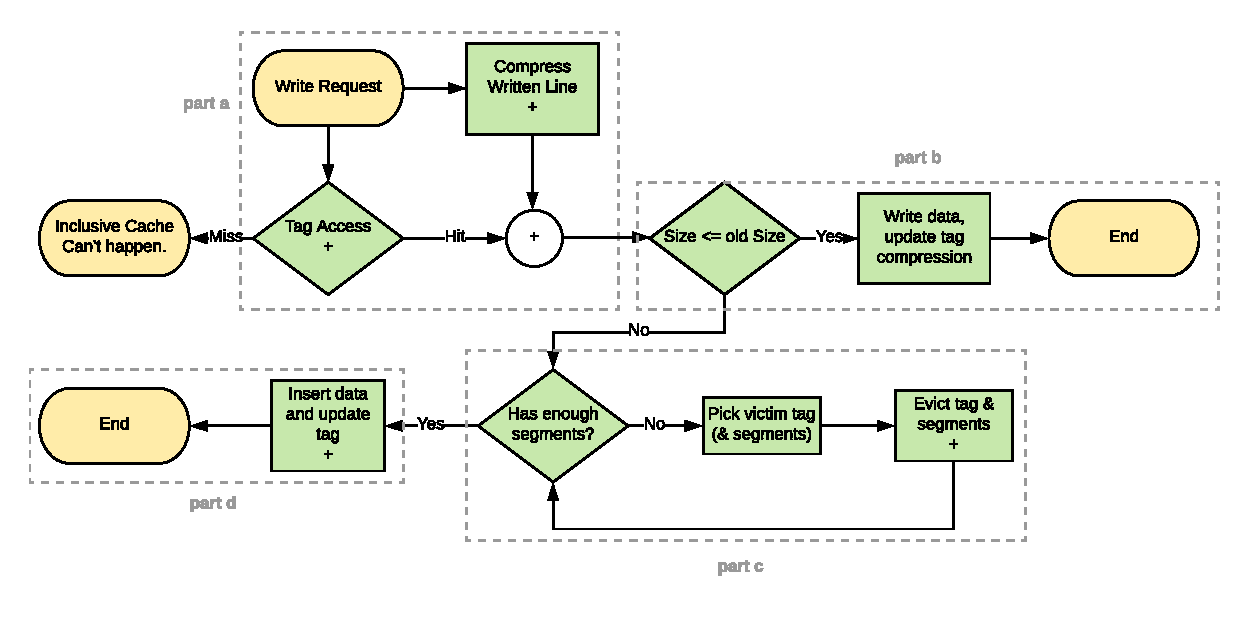
\includegraphics[width=\textwidth,height=\textheight]{BDI_Write.pdf}
    \label{fig:BDI_Write}
    \caption[BDI Write]{Write access flowchart.}
\end{figure}
\begin{figure}
    \contcaption{The flowchart shows the sequence of actions triggered by a write access to the BDI cache. All the blocks are shaded in green because any write request should be off the critical path of the processor regardless of it's status in the cache (hit or miss). Each + sign in any of the blocks signifies an extra latency for tag array access, data array access, or compression}
\end{figure}
\subsubsection{Tag Miss}
We assume inclusive caches, so a write request can never miss. On a read tag miss, just like a normal cache, a request for the missed address is forwarded to the next cache level. Meanwhile a victim tag line has to be selected according to the tag replacement policy (e.g. LRU) and evicted if necessary. When the requested line comes back it is first compressed, then if the free segments in the current data set (can be known from the compression encoding fields of the tag set we accessed) are enough for the incoming compressed line, the line can be inserted right away, otherwise we keep consulting the tag replacement policy to evict more tags and their associated segments until we have enough sapce, then the line can be inserted.
\subsubsection{Tag Hit}
A tag hit has to be treated differently depending on whether it's a read or write request, a read hit is simple, after accessing the tag, the segment pointer is used to access the data line and service the request, a write hit however can be complicated because it can cause the data line to change and thus change it's compressed size. If the new written size is the same or less than the original size then it can be overwritten right away with the tag updated accordingly, otherwise, the we keep evicting tags and their segments according to the replacement policy until we have enough free segments to write the new data line.

\section{Dedup}
\label{sec:Dedup}
\subsection{Structure}
\label{ssec:DedupStructure}
\subsubsection{Tag Array}
\label{sssec:DedupTag}
\subsubsection{Data Array}
\label{sssec:DedupData}
